\documentclass{article}

\usepackage[utf8]{inputenc}
\usepackage[francais]{babel}
\usepackage{dirtree}
\usepackage{graphicx}
\usepackage{float}

% elements du titre
\title{Rapport projet 2, TSAT - Solveur SAT/SMT}
\author{T. Stérin, A. Torres}
\date{Mai 2016}


% definition de quelques macros, pour les maths
\newcommand{\litt}{\alpha}
\newcommand{\non}[1]{\overline{#1}}

\begin{document}

\maketitle

\begin{abstract}
TSAT est un solveur SAT/SMT à l'instar de minisat \cite{minisat} qui a pour but de satisfaire des formules logiques qui lui sont données en entrée.
TSAT est écrit en C++ par Tristan Stérin et Alexy Torres--Aurora-Dugo.
Réalisé à l'ENS Lyon pour l'année scolaire 2015-2016 et dans le cadre de la matière ``Projet2'', ce solveur permet de résoudre des formules SAT/SMT sous formes CNF et logique (en appliquant la transformation de Tseitin).
\\ \\
Différentes méthode de résolution ont été implémentées dans TSAT : 
\begin{itemize}
	\item DPLL (Davis–Putnam–Logemann–Loveland) standard \cite{DPLL}.
	\item DPLL avec méthode des litéraux surveillés \cite{WL}.
	\item DPLL avec méthode avec apprentissage de clause \cite{CL}.
\end{itemize}
\end{abstract}
%Un peu de maths en \LaTeX: voici un exemple de clause:
%$$
%\litt_1\lor\non{\litt_2}\lor\litt_4
%$$
%On remarque au passage que $\non{\non{\litt}}$ est pareil que $\litt$.

\section{Organisation du code}
L'organisation du projet est la suivante :
\dirtree{%
    .1 src/.
    .2 BETHeuristic (Classes contenant les stratégies de pari).
    .2 Global (Fichiers source contenant les paramètres du programme).
    .2 NewCore (Noyau TSAT, structures de clause).
    .3 SMT (Noyau SMT).
    .2 Parser (Parseurs CNF et logique).
    .2 RandomSatExpGenerator (Générateur de formules SAT).
    .2 SMTGenerator (FGénérateur de formules SMT).
    .2 main.cpp (Fichier source principal du solveur).
    .2 main.h (En tête du fichier main.cpp).
    .2 Makefile (Fichier de compilation du solveur).
}

\newpage
\section{Formules compatibles}
TSAT accepte différents types de formules en entrée.
\begin{itemize}
    \item Format DIMACS (SAT) de type : \\
    p cnf 2 9\\\
    1 4 -5\\
    4 5 9
    \newline
    \item Format logique (SAT) de type : \\
    $
    1 \Rightarrow 4 \lor 3 \land (5 \Leftrightarrow 4) \land 3
    $
    \newline
    \item Format logique (SMTE) de type : \\
    $
    4 = 3 \land (5 \neq 4)
    $
    \newline
    \item Format logique (SMTC) de type : \\
    $
    f(a) = b \land g(f(f(a)), c) = 5 \land f(b) = g(a, c)
    $
    \newline
    \item Format logique (SMTD) de type : \\
    $
    x4 - x3 = 4 \land x3 < 0 \land x1 - x2 >= 6
    $
\end{itemize}

\section{Choix des patrons de conception}
Le patron de conception en statégies à été retenu pour le développement des heuristiques de pari. Celà permet d'ajouter une heuristique sans modifier le noyau SAT. Ainsi il est aisé de créer une nouvelle classe heuristique et de l'ajouter au programme en l'incluant dans le fichier main.cpp et modifiant quelques lignes de code dans ce fichier.
Cette méthode de conception permet aussi de modifier l'heuristique de pari durant le traitement de la formule.

Nous avons aussi développé les différents parseurs de formule à l'aide de ce patron de conception afin de faciliter l'ajout de nouveaux types de parseurs.
\section{Choix des implémentations}
MAP pour gagner du temps
Files ?
Lien avec SMT?

\section{Détection de l'UIP}

\section{Critique des performances}
La méthode avec apprentissage de clause permet d'obtenir de très bons résultats. Certaine formules alors impossible à traiter à l'aide de DPLL standard et de la méthode avec les litéraux surveillés obtiennent un solution (afféctation ou réponse d'insatisfaisabilité) en un temps très court.

Certaines heuristiques de pari nous donne de meilleurs résultats dans certain cas. Ainsi, RAND permet dans les meilleur cas de satisfaire des formules en moins d'une seconde alors que l'heuristique standard ne me permet pas en moins de dix. Les meilleurs résultats s'obtiennent avec l'heuristique MOMS.

Les optimisations à la compilation (-O3) permettent elles aussi de rendre le solveur beaucoup plus rapide (jusqu'à 70\% plus rapide dans certain cas).
\\
\begin{figure}[h]
    \begin{center}
        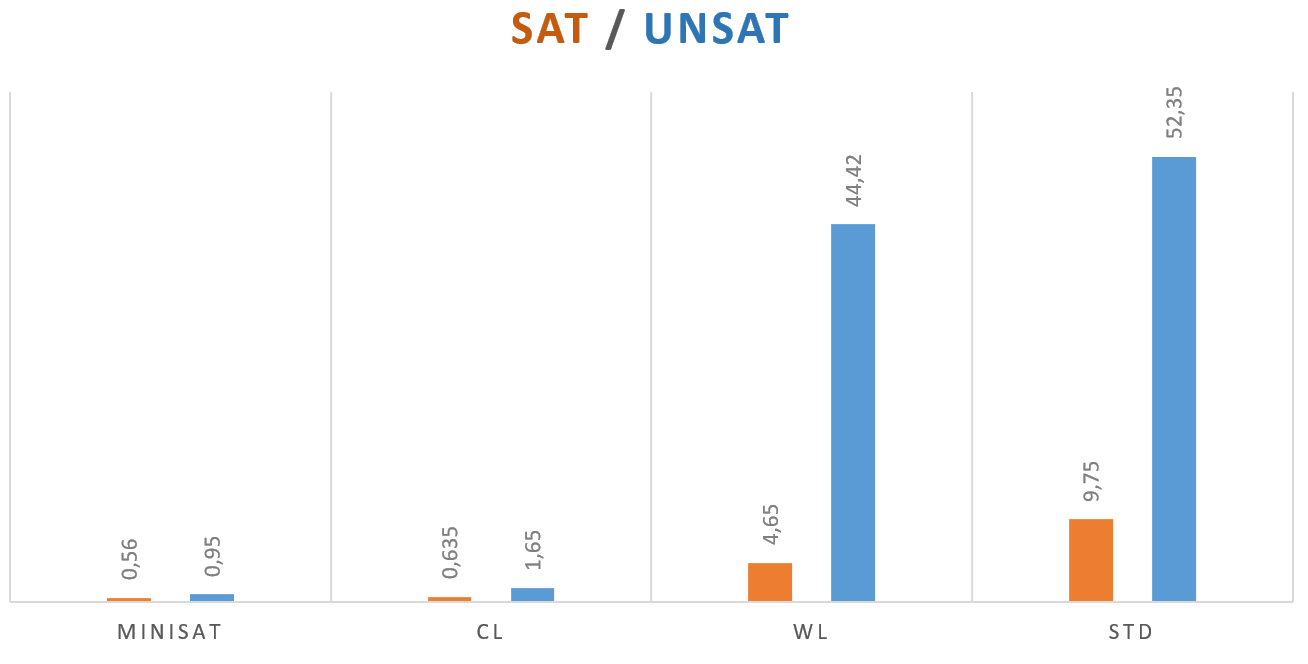
\includegraphics[scale=0.25]{time.png}
    \end{center}
    \caption{Comparaison des temps d'execution de TSAT à MINISAT}
    \label{Comparaisons}
\end{figure}

\section{Améliorations possible}
Plusieurs possibilités d'améliorations sont envisageables, une paraléllisation des tâche peut fournir un apport conssidérable en temps. Une des options pour la parallélisation serait d'exécuter en même temps différentes heuristiques de pari sur la prochaine variable à assigner.

\bibliographystyle{unsrt}
\bibliography{ex-biblio}

\end{document}
